\section{Caso 2. Dos fuentes de datos y dos ontologías.}
\label{section:caso2}

Este caso consiste en la integración e interoperabilidad de dos fuentes con semántica enriquecida por el uso de dos ontologías. Se pretende demostrar la facilidad de realizar consultas a dos fuentes de datos a modo de enriquecer la información obtenida. El caso presenta una situación en el que un mismo proveedor de datos posee dos fuentes de datos distintas, que tienen que interoperar entre si a modo de enriquecer la información obtenida. Este escenario es muy común ya que normalmente aunque nos referimos a un mismo organismo publicador de datos éste posee sistemas de información distintos que pueden o no estar interconectados.


En el capítulo \ref{chap:Implementación de la Ontologia} se desarrolló un sistema que recogió estos datos y los almacenó en dos almacenes de datos distintos y los disponibilizó en dos Puntos SPARQL distintos. En este caso el publicador de los datos es el mismo, pero las ontologías son distintas. Se ejecutó una consulta al Punto SPARQL que utiliza por un lado la ontología de OCDS y los datos de los procesos licitatorios de la DNCP y por otro lado la ontología desarrollada por la DNCP y los datos de Proveedores. En la Figura \ref{img:Diagramacaso2Endpoint} se puede describir gráficamente la situación. Si bien es posible que el mismo proveedor conozca y pueda interconectar internamente entre si ambas fuentes de datos a través de comandos SQL, esto no es verdad para un agente externo de la DNCP, que es el caso dentro de la web semántica, quien no conoce los datos y posee únicamente estos dos puntos de accesos independientes uno de otro.

 \begin{figure}[ht!]
    \centering
    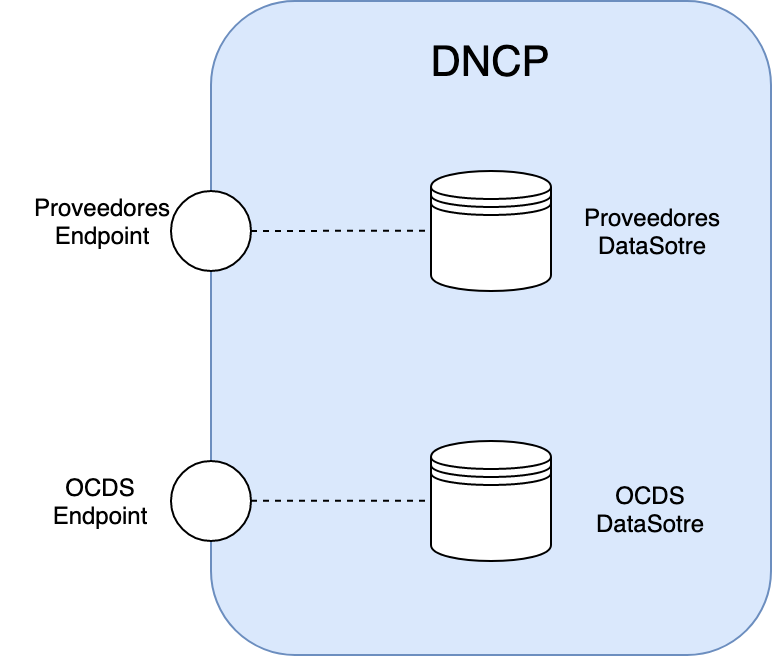
\includegraphics[width=150mm]{figuras/Diagramas-Caso2-Ilustracion.png}
    \caption{Diagrama de fuentes de datos}
    \label{img:Diagramacaso2Endpoint}
 \end{figure}


La consulta presentada en el Cuadro \ref{lst:caso2} consiste en obtener datos de una organización cuyo RUC es 80008004-1. Se utiliza el comando SERVICE para realizar consultas a una fuente de datos distinta indicando su URL.

\noindent\begin{minipage}[c]{\textwidth}
\begin{lstlisting}[captionpos=b, caption={Consulta a dos fuentes de datos}, label={lst:caso2},  numbers=left,  numberstyle=\tiny\color{mygray},frame=single]
SELECT  *
    WHERE {   
            { 
                SELECT DISTINCT   ?c ?d
                WHERE { 
                    ?organization rdf:type          ocds:Organization ;
                                  ocds:identifier   ?identifier .
                    ?identifier   ocds:identifierId "80008004-1" .
                    ?organization ?a                ?b
                    OPTIONAL { 
                        ?b  ?c  ?d 
                    }
                  }
            }
            UNION {
                SERVICE <http://localhost:3030/proveedores_completas_no_inf/sparql>
                  {  ?empresa rdf:type dncp:Proveedor ;
                              dncp:ruc "80008004-1" ;
                              ?x       ?y
                  }
            }
    }
    
 \end{lstlisting}
\end{minipage}

 En la Figura \ref{img:caso2Resultado} se observan en la columna izquierda los datos obtenidos a partir de los Procesos Licitatorios utilizando la ontología OCDSPY y en la columna derecha se observan los datos obtenidos a partir de la fuente de datos de Proveedores que utiliza la ontología de la DNCP.


 \begin{figure}[ht!]
    \centering
    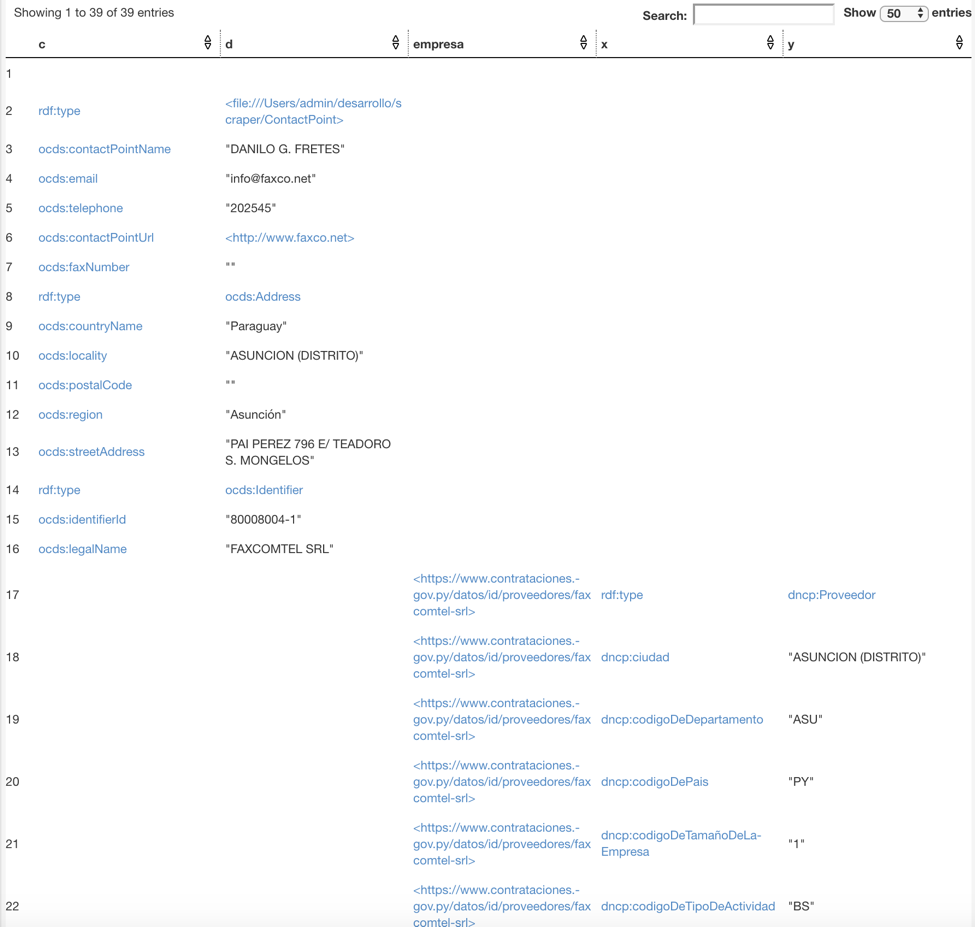
\includegraphics[width=150mm]{figuras/caso2Resultado.png}
    \caption{Despliegue de resultado de la consulta del caso 2}
    \label{img:caso2Resultado}
 \end{figure}



A continuación se presentan las mejoras obtenidas con relación a los datos publicados en el portal de datos de la DNCP.
 
 \subsection{Mejora 1: Igualdad semántica de propiedades}
 Se puede observar que ambas fuentes de datos se relacionan entre sí a partir de la propiedad \textit{ocds:identifierId} y \textit{dncp:ruc}. Sin bien es posible realizar esta relación debido a que un experto de dominio puede deducir que ambas propiedades denotan los mismos valores, esta igualdad no está explícitamente definida en la ontología. 
 
 En el caso que se desee expresar de manera explícita esta información bastaría agregar la propiedad \textit{owl:equivalentProperty}  a la definición de la propiedad \textit{identifierId}. Un ejemplo de cómo quedaría la definición de la propiedad \textit{identifierId} puede verse en el Cuadro \ref{lst:caso2-2}. Con esto es posible utilizar indistintamente cualquiera de las dos propiedades para referirse a la misma relación.\hfill \break

\noindent\begin{minipage}{\textwidth}
 \begin{lstlisting}[captionpos=b, caption={Declaración de equivalencia semántica entre dncp:ruc y ocds:identifierID}, label=lst:caso2-2,  numbers=left,  numberstyle=\tiny\color{mygray},frame=single]
###  http://purl.org/onto-ocds/ocds#identifierId
:identifierId rdf:type owl:DatatypeProperty ,
                        owl:FunctionalProperty ;
                owl:equivalentProperty dncp:ruc ;
                rdfs:domain :Identifier ;
                rdfs:range xsd:integer ,
                            xsd:string ;
                rdfs:comment "The identifier of the organization in the selected scheme."@en ;
                rdfs:label "Identifier ID"@en .
 \end{lstlisting}
\end{minipage}

 Las propiedades equivalentes (\textit{owl:equivalentProperty}) tienen los mismos valores, pero pueden ser semánticamente diferentes, en este caso \textit{dncp:ruc} y \textit{ocds:identifierId} tienen el mismo valor, y \textit{dncp:ruc} se refiere al “Código Único del Contribuyente (RUC) de la Secretaría de Estado y Tributación (SET)” y \textit{ocds:identifierID} se refiere al “Identificador Único de la Organización”. Equivalencia no quiere decir que sean iguales. Para indicar que dos propiedades son iguales se debe utilizar la propiedad \textit{owl:sameAs}
 En la Tabla \ref{table:semanticaID} se expresa la comparación entre las propiedades mencionadas.

 \begin{table}[!htb]
    \centering
    \caption{Definición Semántica de Indentificador y RUC}
    \label{table:semanticaID}
    \resizebox{15cm}{!} {
    \begin{tabular}{|c|l|l|}
    \hline
    
Propiedad & Valor &  Significado \\ \hline

ocds:identifierID  & 80008004-1 &  Identificador de la Organización \\ \hline
dncp:ruc & 80008004-1 &  Código Único del Contribuyente de la Secretaría de Estado y Tributación \\ \hline

    \end{tabular}
    }
    \end{table}
    
 Sin Embargo, Que dos individuos tengan una propiedad con el mismo valor no necesariamente implica que se trate del mismo individuo. En ontologías, a menos que haya una sentencia que indique que dos individuos son iguales o diferentes, no se puede asumir ninguna de las dos situaciones. Esto situación da pie a la mejora 2.

 \subsection{Mejora 2: Igualdad semántica de instancias}
 \label{section:caso2mejora2}
 Como en la fuente de datos no está definida la equivalencia entre ambas instancias, entonces los datos obtenidos de las distintas fuentes deben ser asumidos como iguales por el conocimiento del experto de dominio. La forma de expresar explícitamente la igualdad semántica entre dos instancias seria agregando la sentencia de Cuadro \ref{lst:caso2-1}. En la Figura \ref{img:DiagramaCaso3} se observa como quedaría esta unión semántica entre ambas instancias. Esto aseguraría de que una maquina pueda interpretar la equivalencia entre ambas instancias. 
 
 
\noindent\begin{minipage}[c]{\textwidth}
    \begin{lstlisting}[captionpos=b, caption=Declaración de igualdad semántica de dos instancias, label=lst:caso2-1,  numbers=left,  numberstyle=\tiny\color{mygray},frame=single]
<http://www.contrataciones.gov.py/datos/api/v2/doc/proveedores/ruc/80008004-1> 
owl:sameAs <http://www.contrataciones.gov.py/datos/id/proveedores/fax-comtel-srl>  .

     \end{lstlisting}
\end{minipage}
     \begin{figure}[ht!]
        \centering
        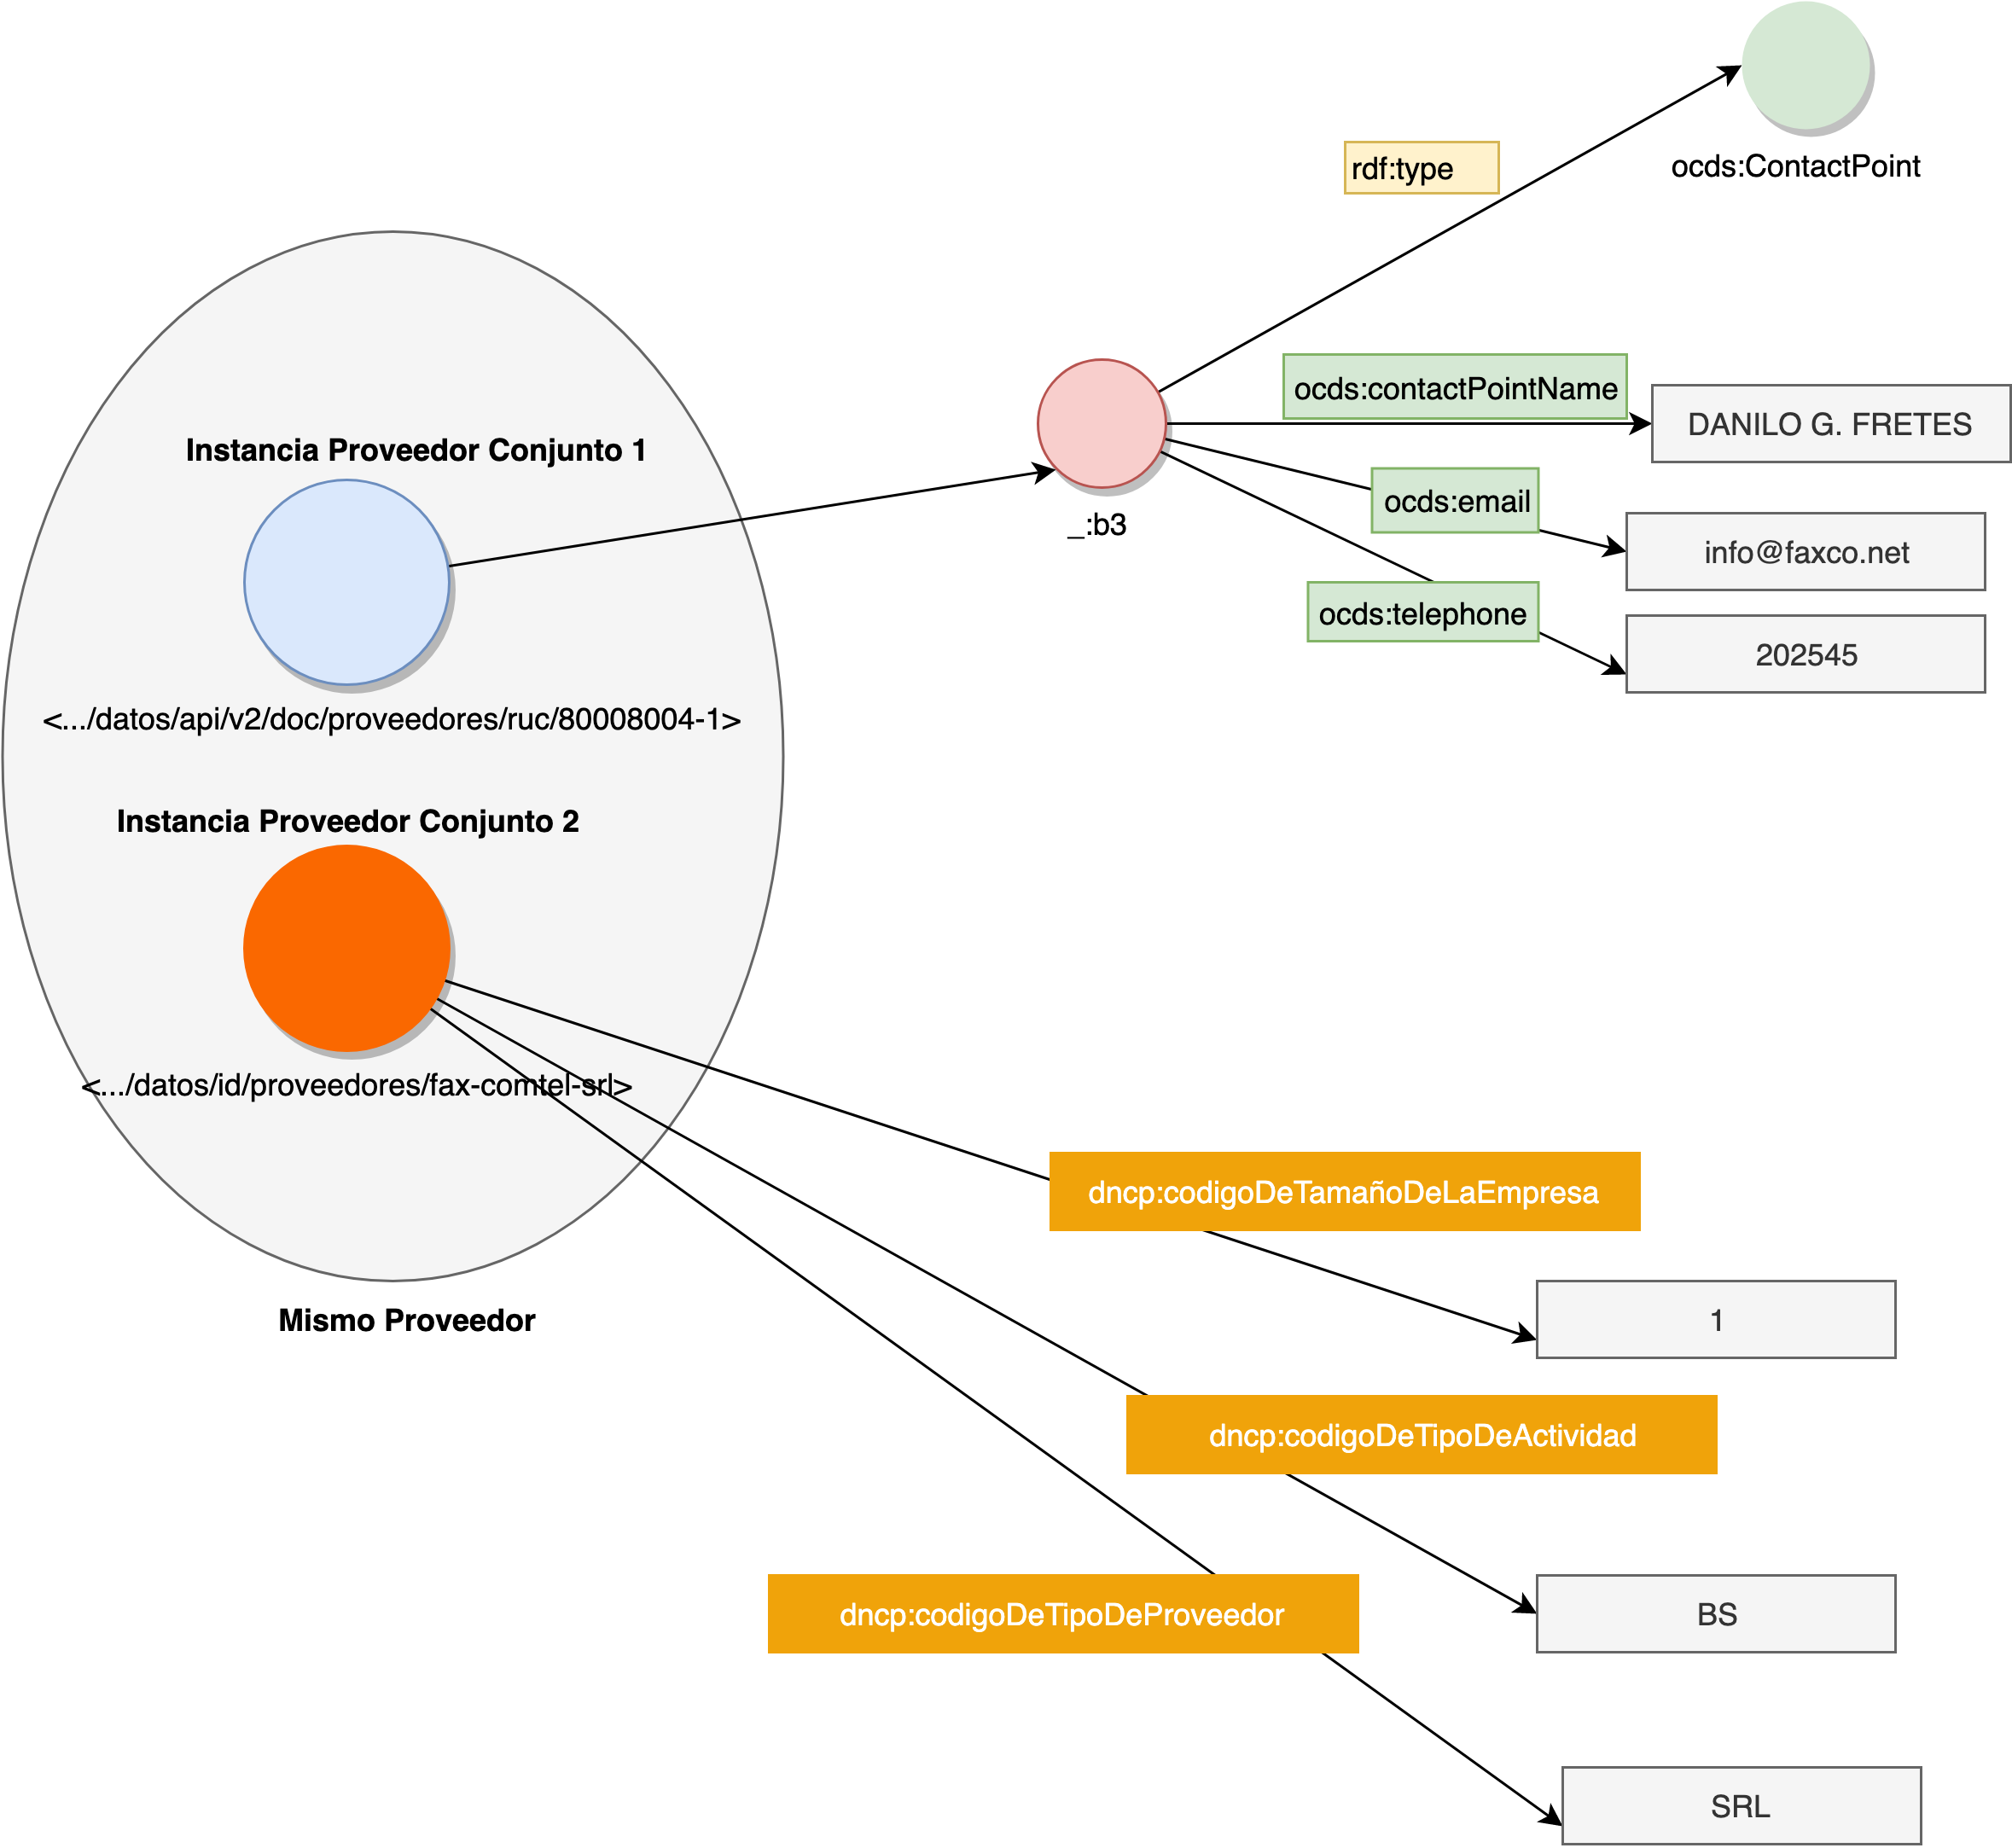
\includegraphics[width=150mm]{figuras/Diagramas-Caso2.png}
        \caption{Grafo de la consulta del caso 2}
        \label{img:DiagramaCaso2}
     \end{figure}

Cabe mencionar, que no se debe hacer una cambio de la sintaxis o de la estructura de los mismos, que podría hacerse llamando a ambas instancias o propiedades con el mismo identificador o mismo nombre de propiedad, sino que solamente bastará por hacer esa conexión semántica.

En este caso se observa que ambos conjuntos de datos pertenecen al mismo Proveedor/Publicador y los datos de las organizaciones se complementan en cuanto a información se refiere. Por una parte podemos obtener datos como el nombre del punto de contacto (\textit{ocds:contactPointName}), email y teléfono. Por otra parte se pueden obtener datos como el código de tipo de proveedor, el cual en este ejemplo es “SRL”. 

    